\chapter[Il concetto di geo-potenziale condizionato e il modello fp-HDGM]{Il concetto di geo-potenziale condizionato e definizione del modello fp-HDGM}
In questo capitolo, viene introdotto il concetto di geo-potenziale condizionato, delineando le sue distinzioni rispetto al geo-potenziale puro. Successivamente, si procede con la presentazione del \textit{Functional Potential Hidden Dynamic Geostatistical Model} (\textit{fp-HDGM}), il quale rappresenta un'estensione del modello f-HDGM per l'analisi dei dati spazio-temporali con interazioni tra le stazioni di osservazione. In questo contesto, vengono esplicitate le equazioni del modello e i parametri da stimare. Infine, viene condotta la simulazione di un modello fp-HDGM al fine di concretizzare i concetti trattati nel capitolo.

\section[Il geo-potenziale condizionato]{Il geo-potenziale condizionato}
Un modello geo-statistico per l'analisi di dati nello spazio per i quali non esiste solo una correlazione spaziale, ma anche un'interazione tra punti di misura, è il \textit{Potential Geostatistical Model} (\textit{GPM})~\cite{paper_GPM}.
\par Sia $\mathbf{s} = (s_{lon}, s_{lat})^\top\in\mathbb{S}^2$ un generico punto spaziale e sia $\mathcal{S} = \{\mathbf{s}_1, \ldots, \mathbf{s}_ N\}$ l'insieme dei punti appartenenti alla regione $D\subset\mathbb{S}^2$ nei quali è stata misurata la variabile d'interesse al tempo $t$ e istante $l$ del dominio funzionale $\mathcal{L}$. La funzione di interazione è così descritta:
\begin{equation}
	p(\mathbf{s}, l, t| \mathcal{S}) = f(\mathbf{s}, l, t) \cdot h_\rho(\mathbf{s}| \mathcal{S});
	\label{funzione di interazione}
\end{equation}
\begin{equation}
	h_\rho(\mathbf{s}|\mathcal{S}) = \left(1 + \sum_{\mathbf{s}' \in \mathcal{S}} f_\rho(\mathbf{s}, \mathbf{s}')\right)^{-1};
	\label{funzione di interazione_2}
\end{equation}
\begin{equation}
	f_\rho(\mathbf{s}, \mathbf{s}') = f_\rho(\|\mathbf{s} - \mathbf{s}'\|) = \exp\left(-\frac{{\|\mathbf{s} - \mathbf{s}'\|}}{{\rho}}\right).
	\label{nonnegative binary function}
\end{equation}
Nello specifico:
\begin{itemize}
	\item $f(\mathbf{s}, l, t)$ è il potenziale di un campo casuale spaziale definito in una regione  $D \subset \mathbb{S}^2$, al tempo $t$ e istante $l$ del dominio funzionale $\mathcal{L}$;
	\item $f_\rho(\|\mathbf{s} - \mathbf{s}'\|)$ è una funzione non negativa definita da $\mathbb{S}^2\times\mathbb{S}^2$ a $\mathbb{R}^+$;
	\item $\|\mathbf{s} - \mathbf{s}'\|$ è la distanza geodetica tra due punti nello spazio;
	\item infine, $\rho \in \mathbb{R}^+$ è il parametro che descrive la forza dell'interazione tra i punti di misura nella regione spaziale $D$.
\end{itemize}
Per comprendere appieno il comportamento della funzione in esame, esploriamo i suoi valori limite. Innanzitutto, si consideri il parametro $\rho$ fissata la distanza geodetica $\|\mathbf{s} - \mathbf{s}'\|$; si osserva che:
\begin{equation}
	\lim_{\rho \to 0} f_\rho(\|\mathbf{s} - \mathbf{s}'\|) = 0
		 \Rightarrow \lim_{\rho \to 0} p(\mathbf{s}, l, t| \mathcal{S}) = f(\mathbf{s}, l, t); \label{limite_per_rho_tendente_a_0}
\end{equation}
\begin{equation}
	\lim_{\rho \to \infty} f_\rho(\|\mathbf{s} - \mathbf{s}'\|) = 1
	\Rightarrow \lim_{\rho \to \infty} p(\mathbf{s}, l, t| \mathcal{S}) = f(\mathbf{s}, l, t)\cdot\frac{1}{N + 1} .
	\label{limite_per_rho_tendente_a_inf}
\end{equation}
Quando $\rho$ tende ad assumere il valore minimo del dominio di definizione (espressione~\ref{limite_per_rho_tendente_a_0}), la funzione di interazione spaziale $h_\rho(\mathbf{s};\mathbf{S})$ raggiunge il suo massimo assoluto, ovvero \num{1}, lasciando così il termine $f(\mathbf{s}, l, t)$ inalterato. Viceversa, quando 
$\rho$ tende a infinito (espressione~\ref{limite_per_rho_tendente_a_inf}), $h_\rho(\mathbf{s};\mathbf{S})$ tende a decrescere fino al suo limite inferiore pari a $\frac{1}{N+1}$, penalizzando significativamente il potenziale puro $f(\mathbf{s}, l, t)$.\par Si consideri ora $\|\mathbf{s} - \mathbf{s}'\|$ fissato $\rho$; si nota che;
\begin{equation}
	\lim_{\|\mathbf{s} - \mathbf{s}' \| \to 0} f_\rho(\|\mathbf{s} - \mathbf{s}'\|) = 1
	\Rightarrow \lim_{\|\mathbf{s} - \mathbf{s}' \| \to 0} p(\mathbf{s}, l, t| \mathcal{S}) = f(\mathbf{s}, l, t)\cdot\frac{1}{N+1};
	\label{limite_per_dist_tendente_a_0}
\end{equation}
\begin{equation}
	\lim_{\|\mathbf{s} - \mathbf{s}' \| \to \infty} f_\rho(\|\mathbf{s} - \mathbf{s}'\|) = 0
	\Rightarrow \lim_{\|\mathbf{s} - \mathbf{s}' \| \to 0} p(\mathbf{s}, l, t| \mathcal{S}) = f(\mathbf{s}, l, t).
	\label{limite_per_dist_tendente_a_infinito}
\end{equation}
Quando $\|\mathbf{s} - \mathbf{s}'\|$ tende a \num{0} (espressione~\ref{limite_per_dist_tendente_a_0}), allora si hanno $N$ stazioni di misura situate nella medesima posizione spaziale; il risultato è l'omogenea ripartizione del potenziale $f(\mathbf{s}, l, t)$ disponibile in $\mathbf{s}$. Invece, quando $\|\mathbf{s} - \mathbf{s}'\|$ tende a infinito (espressione~\ref{limite_per_dist_tendente_a_infinito}), allora i punti di misura sono tra loro indipendenti (assenza di interazione spaziale), di conseguenza il pontenziale $f(\mathbf{s}, l, t)$ rimane invariato.
\par Queste due condizioni estreme forniscono un'importante comprensione del comportamento della funzione di interazione in relazione al parametro $\rho$ e alla distanza geodetica $\|\mathbf{s} - \mathbf{s}'\|$; esse possono avere profonde implicazioni per l'analisi e l'interpretazione del fenomeno studiato.

\subsection[Differenza tra geo-potenziale e geo-potenziale condizionato]{Differenza tra geo-potenziale e geo-potenziale condizionato}
Dopo aver presentato la funzione d'interazione, si è in grado di delineare la seguente divergenza:
\begin{itemize}
	\item il \textbf{geo-potenziale}  $f(\mathbf{s}, l, t)$ è definito come il valore atteso osservato quando $y(\mathbf{s}, l, t)$ viene misurato al tempo $t$ e istante $l$ del dominio funzionale $\mathcal{L}$, nella posizione spaziale $\mathbf{s} \in D$. Esso non è condizionato dalle rilevazioni svolte presso gli altri punti di misura;
	\item il \textbf{geo-potenziale condizionato} $p(\mathbf{s}, l, t)$, invece, è il valore atteso osservato quando $y(\mathbf{s}, l, t| \mathcal{S})$
	viene misurato al tempo $t$ e istante $l$ del dominio funzionale $\mathcal{L}$, nella posizione spaziale $\mathbf{s} \in D$, dato che viene contemporaneamente misurato nella collezione di posizioni $\mathcal{S} = \{\mathbf{s}_1, \ldots, \mathbf{s}_N\}$,  con $s_i \in D, N \geq 1$. Esso è il potenziale spaziale tenente conto anche dell'influenza reciproca esistente tra i punti di osservazione.
\end{itemize}
Si prenda come esempio il potenziale di mercato spaziale in  una rete di attività commerciali anticipato nel capitolo introduttivo. Il geo-potenziale potrebbe dare delle stime promettenti nell'intorno di un generico punto di misurazione $s_i \in\mathcal{S}$, poiché non tiene in considerazione dell'interazione delle altre stazioni di misurazione $\mathbf{s}_1, \ldots, \mathbf{s}_N$, in particolare di $\mathbf{s}_i$. Viceversa, il geo-potenziale condizionato ottiene valori inferiori nell'intorno di $\mathbf{s}_i$ in quanto rappresenta il potenziale che sarebbe osservato con l'aggiunta di una  nuova stazione di misura, se quest'ultima fosse posizionata nelle prossimità di $\mathbf{s}_i$~\cite{paper_GPM}.\par In parole povere, l'apertura di una nuova edicola nelle vicinanze di un'altra preesistente comporterà probabilmente una riduzione delle vendite per entrambe a causa della concorrenza tra attività commerciali. Tale osservazione è fondamentale per comprendere il motivo per il quale il modello f-HDGM dev'essere esteso affinché tenga in considerazione il geo-potenziale condizionato e, di conseguenza, possa essere utilizzato per modellare contesti in cui c'è concorrenza commerciale (e non solo).

\section[Il modello fp-HDGM]{Il modello fp-HDGM}
Il Functional Potential Hidden Dynamic Geostatistical Model (fp-HDGM) vuole espandere l'applicazione dell'f-HDGM all'analisi di dati spazio-temporali in cui è presente interazione tra i punti di misurazione. Questo modello parte dal presupposto che il fenomeno oggetto di studio abbia, anche se minima, una componente di interazione tra i punti di osservazione.
\par L'output del processo, indicato come $y(\mathbf{s}, l, t| \mathcal{S})$ rappresenta la rilevazione al tempo $t$ e all'istante istante $l\in\mathcal{L}$, nella posizione spaziale $\mathbf{s} \in D$, simultaneamente misurato nell'insieme di punti $\mathcal{S} = \{\mathbf{s}_1, \ldots, \mathbf{s}_N\}$, con $\mathbf{s}_i\in D, N \geq 1$.

\subsection[Equazioni del modello]{Equazioni del modello}
Il nuovo modello proposto viene così definito dalla seguente gerarchia di equazioni:
\begin{equation}
	y(\mathbf{s}, l, t| \mathcal{S}) = w(\mathbf{s}, l, t)\cdot h_\rho(\mathbf{s}|\mathcal{S});
	\label{eq_rumore_uscita_HDGM}
\end{equation}
\begin{equation}
	w(\mathbf{s}, l, t)= f(\mathbf{s}, l, t) + \epsilon(\mathbf{s}, l, t);
	\label{eq_rumore_uscita_fp_HDGM}
\end{equation}
\begin{equation}
	f(\mathbf{s}, l, t) = \mathbf{x}(\mathbf{s}, l, t)^\top\cdot\boldsymbol{\beta}(l) + \Phi_z(l)^\top\cdot\mathbf{z}(\mathbf{s}, t);
	\label{eq_comp_det_fp-HDGM}
\end{equation}
\begin{equation}
	\mathbf{z}(\mathbf{s}, t) = G\cdot \mathbf{z}(\mathbf{s}, t-1) + \boldsymbol{\eta}(\mathbf{s}, t).
	\label{eq_comp_lat_fp-HDGM}
\end{equation}
Un'osservazione interessante emerge esaminando il modello al variare del parametro $\rho$, secondo le considerazioni fatte riguardo alle equazioni \ref{limite_per_rho_tendente_a_0} e \ref{limite_per_rho_tendente_a_inf}. Nel dettaglio, si nota che:
\begin{equation}
	\lim_{\rho \to 0} y(\mathbf{s}, l, t| \mathcal{S}) = w(\mathbf{s}, l, t). \label{limite_geo-potenziale_condizionato_rho_a_0}
\end{equation}
Questa osservazione porta a vedere il modello f-HDGM come un caso particolare di quello nuovo, ovvero con $\rho=0$.

\subsection[Parametri da stimare]{Parametri da stimare}
In definitiva, si presenta il vettore dei parametri $\psi$ da stimare di dimensione $n_\epsilon + n_\beta\cdot b + 3\cdot n_z+1$:
\begin{equation}
	\boldsymbol{\psi} = (\mathbf{c}_\epsilon^\top, \mathbf{c}_\beta^\top, \mathbf{g}^\top, \mathbf{v}^\top, \boldsymbol{\theta}^\top, \rho)^\top.
\end{equation}
Analogamente a come precedentemente discusso per il modello f-HDGM, non tutti i parametri possono essere stimati attraverso formule chiuse, ma necessitano di essere risolti mediante ottimizzazione numerica.

\paragraph[Differenza tra correlazione spaziale e interazione spaziale]{Differenza tra correlazione spaziale e interazione spaziale} Nonostante $\theta$ e $\rho$ siano parametri dalla stessa funzione\footnote{$f_i(\|\mathbf{s} - \mathbf{s}'\|)=\exp(-\frac{\|\mathbf{s} - \mathbf{s}'\|}{i})$.}, essi differiscono nel loro scopo fondamentale. $\theta$ è progettato per modellare l'interazione naturale tra tutti i punti nello spazio, ovvero la correlazione spaziale, mentre $\rho$ insiste sull'interazione tra le stazioni di misura presenti nello spazio. 
In termini chiari, il parametro $\theta$ condiziona entrambi i geo-potenziali, viceversa $\rho$ influenza solo il geo-potenziale condizionato.

\subsection[Simulazione di una mappa di geo-potenziale]{Simulazione di una mappa di geo-potenziale}
Al fine di concretizzare le nozioni riportate nel capitolo, con l'utilizzo del software MATLAB, è stata compiuta una simulazione della realizzazione di un processo descritto secondo un fp-HDGM. La simulazione è stata condotta nell'area della provincia di Bergamo. Per garantire la pertinenza del caso di studio con un contesto realistico, sono stati distribuiti i punti di misurazione in cluster localizzati in alcune aree urbane della provincia (figura~\ref{mappa_stazioni_simulate}). 
\begin{figure}[htp]
	\centering
	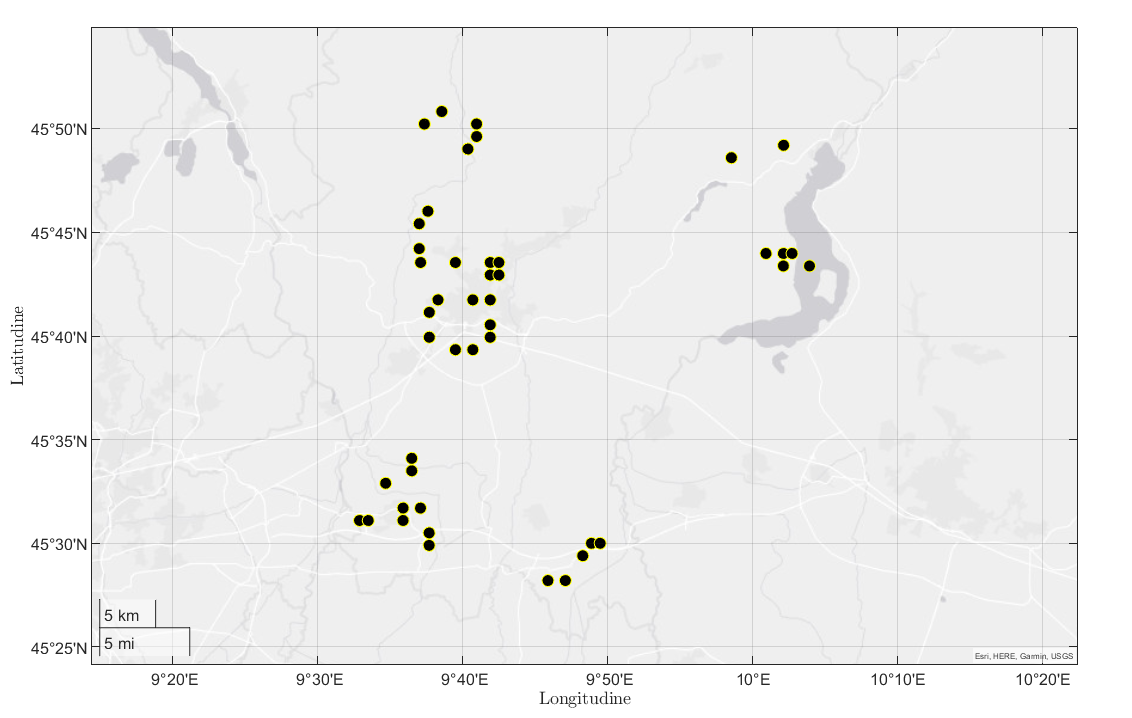
\includegraphics[height=260px]{Immagini/2. Nuovo modello/Mappa stazioni simulate_png}
	\caption[Collocazione spaziale dei punti di misura della simulazione.] {collocazione spaziale dei punti di misura della simulazione. Sono stati definiti 7 cluster di stazioni di misurazione nei comuni di Bergamo, Treviglio, San Pellegrino Terme, Sovere, Sorisole, Antegnate e Parzanica di numerosità pari a \num{15}, \num{10}, \num{5}, \num{2}, \num{3}, \num{5} e \num{5} rispettivamente.}
	\label{mappa_stazioni_simulate}
\end{figure}
Di seguito è riportata la numerosità dei parametri scelti per la simulazione:
\begin{itemize}
	\item numero di stazioni di misura, $n=45$;
	\item numero di covariante globali, $b=1$;                               
	\item dimensione del dominio funzionale ad alta frequenza, $q=24,\ \mathcal{L}=[0, 23]$;
	\item numero di campioni in bassa frequenza, $T=365$;
	\item numero di funzioni base utilizzate per modellare  $\sigma_\epsilon (l)$,  $n_\epsilon =5$;
	\item numero di funzioni base utilizzate per modellare $\beta(l)$, $n_\beta=5$;
	\item numero di funzioni base utilizzate per modellare $\Phi_z(l)$, $n_z=5$.
\end{itemize}
Infine, si espongono i valori fissati del set di parametri:
\begin{itemize}
	\item $\rho = \SI{1100}{\meter}$;
	\item $\mathbf{c}_\epsilon = \begin{bmatrix} 2 & -2 & -10 & 0.5 & 2 \end{bmatrix}$;
	\item $\mathbf{c}_\beta = \begin{bmatrix} 2 & 4 & 8 & 0.5 & 2 \end{bmatrix}$;
	\item $\boldsymbol{\theta} = \begin{bmatrix} 0.05 & 0.05  & 0.05 & 0.05  & 0.05  \end{bmatrix}$;
	\item $G = 
	\begin{bmatrix}
		0.26 & 0 & 0 & 0 & 0 \\
		0 & 0.41 & 0 & 0 & 0 \\
		0 & 0 & 0.6 & 0 & 0 \\
		0 & 0 & 0 & 0.26 & 0 \\
		0 & 0 & 0 & 0 & 0.6 \\
	\end{bmatrix};
	$
	\item $V = 
	\begin{bmatrix}
		8 & 0 & 0 & 0 & 0 \\
		0 & 3 & 0 & 0 & 0 \\
		0 & 0 & 2 & 0 & 0 \\
		0 & 0 & 0 & 3 & 0 \\
		0 & 0 & 0 & 0 & 4 \\
	\end{bmatrix}.
	$
\end{itemize}
Una volta eseguita la simulazione del processo, è stata applicata la tecnica di Kriging\footnote{Il kriging è un metodo di regressione usato in geo-statistica che, minimizzando l'errore quadratico medio, permette di interpolare una grandezza nello spazio. In questo caso, consente di stimare il geo-potenziale.} allo scopo di rappresentare la mappa del potenziale condizionato al variare del parametro $\rho$. Da sottolineare la circostanza con $\rho = 0$, ossia il caso in cui il geo-potenziale condizionato è pari al geo-potenziale puro per le considerazioni fatte sul limite~\ref{limite_geo-potenziale_condizionato_rho_a_0}.

\begin{figure}[h!]
	\centering
	\subfigure[]{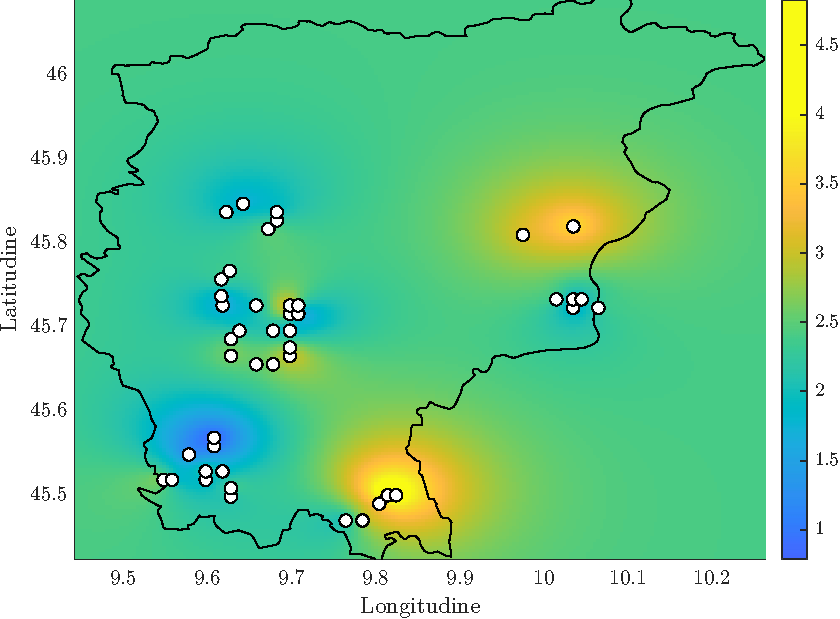
\includegraphics[height=150px]{Immagini/2. Nuovo modello/Mappa potenziale, rho = 0}\label{sim_fp-HDGM_a}}\quad
	\subfigure[]{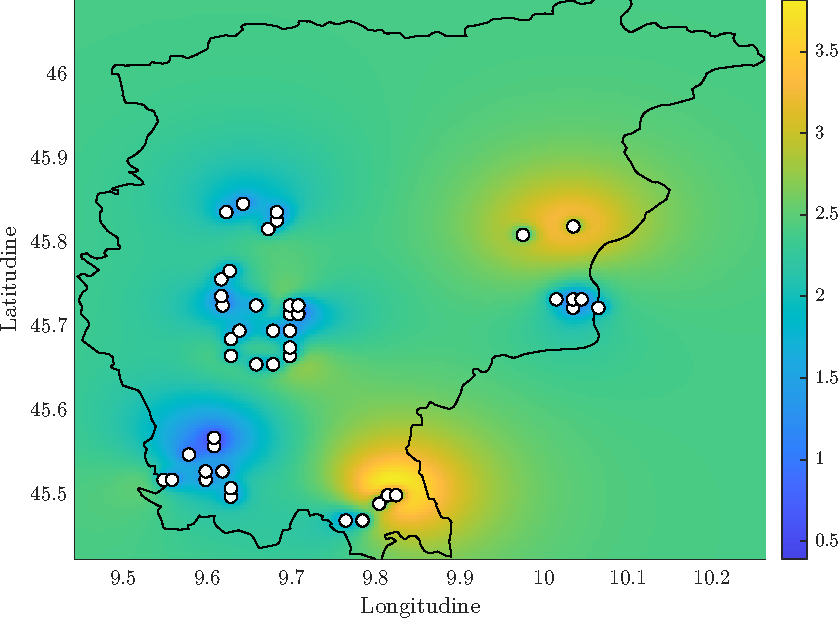
\includegraphics[height=150px]{Immagini/2. Nuovo modello/Mappa potenziale, rho = 0.005}\label{sim_fp-HDGM_b}}\quad
	\subfigure[]{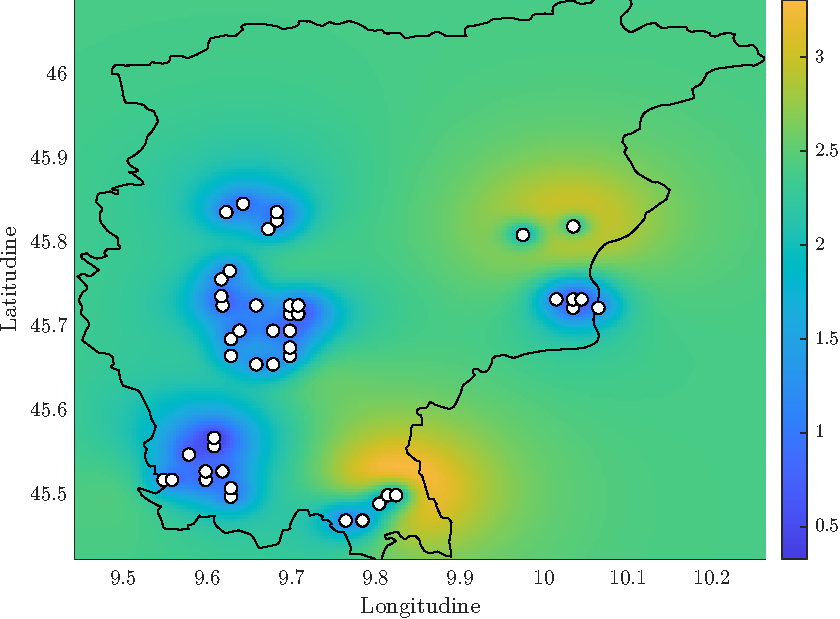
\includegraphics[height=150px]{Immagini/2. Nuovo modello/Mappa potenziale, rho = 0.01}\label{sim_fp-HDGM_c}}\quad
	\subfigure[]{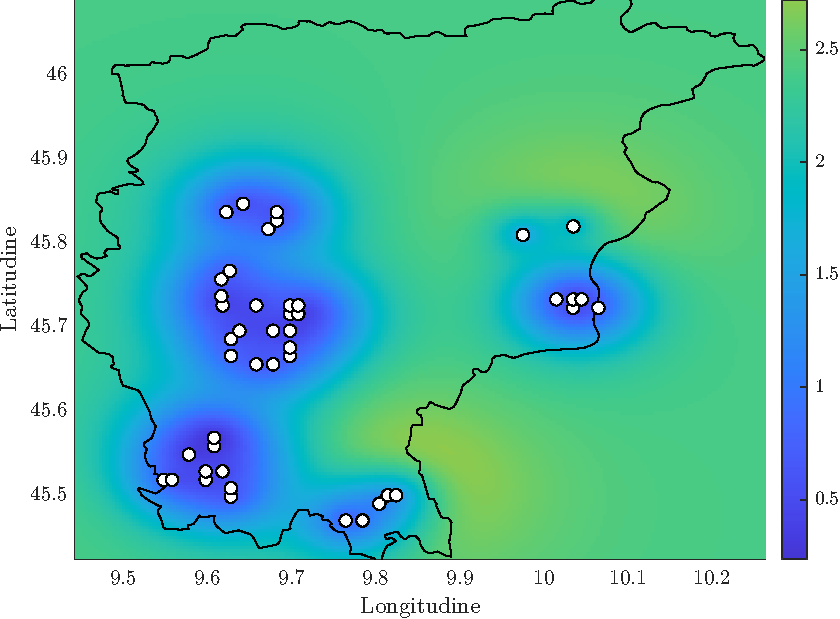
\includegraphics[height=150px]{Immagini/2. Nuovo modello/Mappa potenziale, rho = 0.02}\label{sim_fp-HDGM_d}}\quad
	\caption[Simulazione di un processo fp-HDGM al variare di $\rho$]{simulazione di un processo fp-HDGM, fissati gli indici $l$ e $t$, con $\rho=$ \SI{0}{\meter} (a), \SI{555}{\meter} (b), \SI{1100}{\meter} (c) e \SI{2200}{\meter} (d).}
	\label{sim_fp-HDGM}
\end{figure}
Nella figura~\ref{sim_fp-HDGM} si osserva come il geo-potenziale condizionato diminuisca all'aumentare di $\rho$, specialmente nelle zone con una forte densità di stazioni di misurazione. Si prenda ora come ipotesi che le stazioni di misurazione possano rappresentare dei punti di vendita di un prodotto; valgono le considerazioni fatte riguardo al potenziale di mercato spaziale. Infatti, se si decidesse di aggiungere un punto di vendita nei pressi delle coordinate $(\SI{45.75}{\degree} \text{N}, \SI{9.70}{\degree} \text{W})$, il geo-potenziale puro previsto in questa area risulta essere promettente ma forviante in quanto vicino ad altri punti di vendita, figura~\ref{sim_fp-HDGM_a}. Con $\rho \geq \SI{555}{\meter}$, figure~\ref{sim_fp-HDGM_b}, \ref{sim_fp-HDGM_c} e \ref{sim_fp-HDGM_d}, è facile osservare che il geo-potenziale condizionato è previsto basso nell'area presa in esame, ovvero il punto di vendita verrebbe collocato in un'area caratterizzata da un basso potenziale di mercato spaziale.